\documentclass{sigchi}

% Use this section to set the ACM copyright statement (e.g. for
% preprints).  Consult the conference website for the camera-ready
% copyright statement.

% Copyright
\CopyrightYear{2018}
%\setcopyright{acmcopyright}
\setcopyright{acmlicensed}
%\setcopyright{rightsretained}
%\setcopyright{usgov}
%\setcopyright{usgovmixed}
%\setcopyright{cagov}
%\setcopyright{cagovmixed}
% DOI
\doi{http://dx.doi.org/10.475/123_4}
% ISBN
\isbn{123-4567-24-567/08/06}
%Conference
\conferenceinfo{CHI'16,}{May 07--12, 2016, San Jose, CA, USA}
%Price
\acmPrice{\$15.00}

% Use this command to override the default ACM copyright statement
% (e.g. for preprints).  Consult the conference website for the
% camera-ready copyright statement.

%% HOW TO OVERRIDE THE DEFAULT COPYRIGHT STRIP --
%% Please note you need to make sure the copy for your specific
%% license is used here!
% \toappear{
% Permission to make digital or hard copies of all or part of this work
% for personal or classroom use is granted without fee provided that
% copies are not made or distributed for profit or commercial advantage
% and that copies bear this notice and the full citation on the first
% page. Copyrights for components of this work owned by others than ACM
% must be honored. Abstracting with credit is permitted. To copy
% otherwise, or republish, to post on servers or to redistribute to
% lists, requires prior specific permission and/or a fee. Request
% permissions from \href{mailto:Permissions@acm.org}{Permissions@acm.org}. \\
% \emph{CHI '16},  May 07--12, 2016, San Jose, CA, USA \\
% ACM xxx-x-xxxx-xxxx-x/xx/xx\ldots \$15.00 \\
% DOI: \url{http://dx.doi.org/xx.xxxx/xxxxxxx.xxxxxxx}
% }

% Arabic page numbers for submission.  Remove this line to eliminate
% page numbers for the camera ready copy
% \pagenumbering{arabic}

% Load basic packages
\usepackage{balance}       % to better equalize the last page
\usepackage{graphics}      % for EPS, load graphicx instead 
\usepackage[T1]{fontenc}   % for umlauts and other diaeresis
\usepackage{txfonts}
\usepackage{mathptmx}
\usepackage[pdflang={en-US},pdftex]{hyperref}
\usepackage{color}
\usepackage{booktabs}
\usepackage{textcomp}

% Some optional stuff you might like/need.
\usepackage{microtype}        % Improved Tracking and Kerning
% \usepackage[all]{hypcap}    % Fixes bug in hyperref caption linking
\usepackage{ccicons}          % Cite your images correctly!
% \usepackage[utf8]{inputenc} % for a UTF8 editor only

% If you want to use todo notes, marginpars etc. during creation of
% your draft document, you have to enable the "chi_draft" option for
% the document class. To do this, change the very first line to:
% "\documentclass[chi_draft]{sigchi}". You can then place todo notes
% by using the "\todo{...}"  command. Make sure to disable the draft
% option again before submitting your final document.
\usepackage{todonotes}

% Paper metadata (use plain text, for PDF inclusion and later
% re-using, if desired).  Use \emtpyauthor when submitting for review
% so you remain anonymous.
\def\plaintitle{Focus On Story: Using Narratology-Inspired Lenses to Understand Player Affective Response Data in Choice-Based Interactive Narratives}
\def\plainauthor{First Author, Second Author, Third Author,
  Fourth Author, Fifth Author, Sixth Author}
\def\emptyauthor{}
\def\plainkeywords{Authors' choice; of terms; separated; by
  semicolons; include commas, within terms only; required.}
\def\plaingeneralterms{Documentation, Standardization}

% llt: Define a global style for URLs, rather that the default one
\makeatletter
\def\url@leostyle{%
  \@ifundefined{selectfont}{
    \def\UrlFont{\sf}
  }{
    \def\UrlFont{\small\bf\ttfamily}
  }}
\makeatother
\urlstyle{leo}

% To make various LaTeX processors do the right thing with page size.
\def\pprw{8.5in}
\def\pprh{11in}
\special{papersize=\pprw,\pprh}
\setlength{\paperwidth}{\pprw}
\setlength{\paperheight}{\pprh}
\setlength{\pdfpagewidth}{\pprw}
\setlength{\pdfpageheight}{\pprh}

% Make sure hyperref comes last of your loaded packages, to give it a
% fighting chance of not being over-written, since its job is to
% redefine many LaTeX commands.
\definecolor{linkColor}{RGB}{6,125,233}
\hypersetup{%
  pdftitle={\plaintitle},
% Use \plainauthor for final version.
%  pdfauthor={\plainauthor},
  pdfauthor={\emptyauthor},
  pdfkeywords={\plainkeywords},
  pdfdisplaydoctitle=true, % For Accessibility
  bookmarksnumbered,
  pdfstartview={FitH},
  colorlinks,
  citecolor=black,
  filecolor=black,
  linkcolor=black,
  urlcolor=linkColor,
  breaklinks=true,
  hypertexnames=false
}

% create a shortcut to typeset table headings
% \newcommand\tabhead[1]{\small\textbf{#1}}

% End of preamble. Here it comes the document.
\begin{document}

\title{\plaintitle}

\numberofauthors{3}
\author{%
  \alignauthor{Leave Authors Anonymous\\
    \affaddr{for Submission}\\
    \affaddr{City, Country}\\
    \email{e-mail address}}\\
  \alignauthor{Leave Authors Anonymous\\
    \affaddr{for Submission}\\
    \affaddr{City, Country}\\
    \email{e-mail address}}\\
  \alignauthor{Leave Authors Anonymous\\
    \affaddr{for Submission}\\
    \affaddr{City, Country}\\
    \email{e-mail address}}\\
}

\maketitle

\begin{abstract}
Previous player experience studies involving story-driven games such as modern adventure games have focused on evaluating gameplay-related player feelings such as agency, transportation or immersion, but none have focused on the core of story-driven games: emotional engagement with the story. We ra-n a study with 7 subjects playing a contemporary interactive narrative and recorded physiological measurements, the Sensual Evaluation Instrument (SEI) use, and facial expression recognition. Our goal was to trace individual player relationship patterns between affective responses and story elements. Therefore we developed several features derived from narratology and screenwriting craft to analyze the data collected from the perspective of plot, character, and values. We tagged annotations of videos in order to analyze player choices and affective responses using these three approaches. We argue that leveraging a narrative-based content analysis of a narrative game provides deeper insight into quantitative player experience data.
\end{abstract}

\category{H.5.2.}{Information Interfaces and Presentation: User InterfaceS: Evaluation/methodology; 1.2.1 Applications and Expert Systems: Games.}{Miscellaneous}{}{}

\keywords{Game user research; narrative; content analysis; narratology; adventure games; story}

\section{Introduction}
\label{sec:orgdbcc5cd}
Stories are designed to elicit emotional responses and to engage their
audience. Modern adventure games, particularly those defined by game
developer Telltale Games, have evolved the traditional puzzle-focused
story game closer to the types of experiences found in television and
film, both in content and in presentation \cite{Parker2013-el}. These
games take advantage of licensed content to tell stories using a
combination of interesting choices and participatory action sequences
(known commonly as quick-time events (QTE)). The experience players
have of these games is inseparable from the story itself, and
represent a good example of combining stories and games. Unlike many
games, the player experience in this genre derives from the narrative
content portrayed and within which player actions are
contextualized. This motivates our present paper's proposed
methodology of using a content analysis of the work to analyze
recorded player experience data, in particular data relating to
choices and emotions. This paper presents a methodology and its
application of player responses to \emph{The Wolf Among Us} (TWAU) by
Telltale Games \cite{Telltale_Games2013-hz} using three distinct
lenses: values, characters and plot. We use a content encoding schema
to annotate videos with distinct segments of play that correspond to
beats, story events and characters in order to contextualize player
responses using physiological data \cite{Robinson2016-qr}, and use the
Sensual Evaluation Instrument (SEI) to record instances of
self-reported affect \cite{Isbister2006-sc}.

The content of interactive narrative games can be viewed as two
interconnected layers: the ludic layer, whereby the player takes
actions with the goal of achieving some desired outcome, and the
narrative layer, where the work itself exerts structure and has a goal
of creating an effect on the player through the sequence and
presentation of content. They are intertwined in the case of Telltale
games as each choice is necessarily tied to the narrative and not some
underlying simulation. Mawhorter has started formalizing a poetics of
choice to describe the network of meaning and action that comprises
narrative choice-based games \cite{Mawhorter2016-cx}. We draw from his
theory two concepts to evaluate the role that choices play in the
overall narrative (specifically \emph{framing} and \emph{outcomes}) that aid our
analyzing the way that choices operate within this particular
game. Not every decision within the game has the same weight in terms
of the story, and not every emotional moment can be traced to a player
decision, so the narrative layer is characterized by classifying the
timing and content of the narrative itself.

This paper is organized as follows. First, we review related work in
player experience analysis as well as narrative theory and its
applications to interactive narratives. We follow by a description of
the study design and the features that comprise the different
analytical lenses. We then present the results of analyzing the
playthroughs, as well as assessing the underlying distribution of
content. Finally, we discuss the implications and motivate future work
that combines content analysis, modeling and empirical studies.

\section{Background}
\label{sec:org7de9e30}
Player experience evaluation has evolved out of the realization that
the experience of entertainment software is distinct from that of
other types of software \cite{Sanchez2012-cz} [more citations]. The
current state-of-the-art methods include qualitative (surveys and
questionnaires \cite{Qin2009-xm}, think-aloud \cite{Tan2014-xr}, and
interviews) along with quantitative (video analysis of playthroughs
\cite{Marczak2012-bs}, physiological measurements
\cite{Mandryk2006-sd}, and telemetry data \cite{Drachen2015-hn}). We
build on these techniques using a mixed-method approach that borrows
aspects of each to bring to bear on a particular genre of story games.

The exact relationship between games and stories has been the source
of debate in game studies as well as in artificial intelligence. The
focus of the debate has been on whether the traditional methods and
techniques from the study of linear narrative in print and film can be
successfully applied to games, or whether games constitute a unique
artifact deserving of their own field. While this debate has largely
been resolved \cite{Aarseth2012-ol}, the practical question of whether
it was even possible to fuse the two and achieve a high degree of both
story and agency has been a topic of intense research and
experimentation. The benefits of such work advances in personalized
education \cite{Rowe_undated-cl}, and training in addition to the
market in the entertainment sector. One early example which is still
often cited is that of Facade, an interactive drama which uses
real-time sequencing of dramatic beats \cite{Mateas2003-ty}. This work
was also a challenge to evaluate given the experimental nature of
using parser-based input as well as the novelty for players to
experience dynamic content sequencing
\cite{Mehta2007-gn,Seif_El-Nasr2013-hp}.

Other experiments in interactive narrative generation have also been
the source of innovations in evaluation that focus on particular
aspects of the narrative experience, such as surprise
\cite{Bae2014-au,Bae2008-js}, suspense \cite{Cheong2007-ts}, and
emotions \cite{Roberts2009-km}. These rely heavily on games that have
been crafted specifically for the experiment, and use a combination of
methods [detail] to evaluate specific effects that the experimental
games hope to trigger.

Recent work in computational narratology has drawn from linguistic
traditions to model and annotate narratives
\cite{Cataldi_undated-sf,Szilas2010-tg,Finlayson2011-tw} and to collect
these as corpora \cite{Elson2012-xn,Finlayson2013-wi} from which
patterns and theories can be drawn. We use these as inspiration for
their combination of content and interpretation in designing the study
and planning for future use of the dataset for other experiments.

Gameplay telemetry is a valuable source of empirical data and is a
cornerstone of industry assessment of game success
\cite{Drachen2015-hn}. Narrative games have also been the subject of
telemetry assessment \cite{Murtagh2014-wl}. Other approaches focus on
evaluating the properties of the narrative itself
\cite{Szilas2014-fd}. A promising vein of research is the use of
direct measures of brain activity and physiological measurements to
evaluate player engagement with narratives
\cite{Wallentin2011-mq}. These studies suggest that heart rate
variability may be a more relevant measure than heart rate peaks.

One of the closest studies to the present work was completed by
El-Nasr et. al. on Facade using a qualitative analysis. In it, the
authors analyze player behavior, emotion and interpretation using a
variety of methods. Another user study specifically investigating
narrative was conducted by Mallon and Webb \cite{Mallon2005-ck} which
also employed a reader-response approach.

\section{Methodology}
\label{sec:orgd085191}
Game genres differ widely from one another and benefit from a method
specific to their particular characteristics, as Johnson et al show in
their work on the massive online battle arena genre
\cite{Johnson2015-sd}. While narrative games have been the focus of
evaluation in the past, the story has been either a secondary concern
(in the case of adventure games \cite{Mallon2005-ck} used a similar
reader-response approach, with a more bottom-up method and a broader
scope). In generative works, the evaluation has focused on the results
of the method of generation, as in Mawhorter's experiments with
creating choice structures \cite{Mawhorter2013-ym,Szilas2014-fd}, or
the interface itself \cite{Mehta2007-gn}.

We want to focus on the affective effects of narrative games, or in
literary terms, the "reader response" aspects, making Telltale-style
adventure games an appropriate object of study, since they do not
employ in their currently published games algorithmic story generation
or presentation. Therefore analyzing a player experience would benefit
from techniques and concepts drawn from narratology and screenwriting
theory. The primary content in such games is often linear and the
primary value cited in popular reviews of its games are its compelling
characters, interesting story and meaningful decisions
\cite{Macgregor2015-do}, while its detractors often cite limited
variation in plot as betraying the promise at the beginning of each
Telltale Game: "This game series adapts to the choices you make. The
story is tailored by how you play”. We have developed a methodology
that focuses on player response based on the underlying narrative
content and the principle mechanic of the genre, player choices.

\subsection{Content Analysis and Measures of Player Affect}
\label{sec:org6be524e}

The primary goal was to understand the relationships between the
player's emotional response and the narrative elements that gave rise
to them. Narrative and story are considered a complex mental
capability \cite{Herman2013-ab} and a privileged mode of discourse ,
it is also a primary focus of many game designers and studios
\cite{Salter2017-mp} and has a continued popularity in the educational
sector \cite{Rowe2009-pv}. A secondary goal was to compare objective
metrics of individual player experiences and emotional response
through different paths of a dynamic story that was being encountered
for the first time. We were interested in both effects caused by the
story itself as well as the variations in reception that each player
brought to bear. While at some level stories are understood as complex
networks of causal chains and events, they are also a powerful tool
for broadening perspectives and conveying and critiquing
worldviews. \emph{TWAU} exemplifies this in its portrayal of a divided
community that facilitates firsthand emotional experience of prejudice
and mistrust.

We chose \emph{TWAU} for this and due to its critically reception. The game
is a new story set within the comic series Fables by Bill
Willingham. In it the player-character, Bigby, is a sheriff of a
community of fairytale refugees who have fled their homeland. The
story centers around a murder and the subsequent investigation that
highlights class tensions between human and non-human members. The
gameplay consists of both action-oriented sequences (quicktime events)
and timed choices where the player indicates a response for the
player-character, often in the context of an interaction with another
character. These choices and what they express are where much of the
interest in the genre lies, as players are often presented with
ethical dilemmas or charged choices \cite{Nay2017-nt}. Every timed
choice has a default option of silence, which is often interpreted by
the other characters in the game based on what they know of the
character and context. McKee describes dialogue as the surface form of
underlying actions, and further asserts that "not speaking when a
situation calls for talk is an action, perhaps a cruel one, aimed at
another person.”  \cite{Mckee2016-vm}. The fixed timeline of many of
these sequences constrain the overall pace of the game to
approximately two hours.

\subsection{Study Design}
\label{sec:org61d90f3}
We conducted a study ( n= 7) with uncompensated graduate or
undergraduate students. Each participant was instructed to play
through the first episode of TWAU, using several sensors and self
report instruments. These included All the Feels (ATF)
\cite{Robinson2016-qr}, a set of sensors designed to enable bloggers
to broadcast their physiological signs, the Sensual Evaluation
Instruments (SEI) \cite{Isbister2006-sc,Laaksolahti2009-uw}, designed
for nonverbal self-report, and think-aloud techniques. 

\begin{figure}[htbp]
\centering
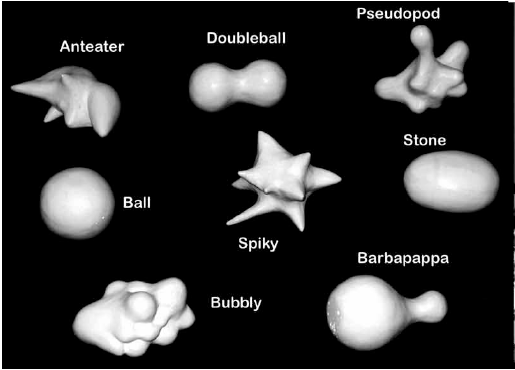
\includegraphics[width=.9\linewidth]{figures/sei.PNG}
\caption{\label{fig:org5b60ba7}
SEI Models}
\end{figure}

We decided on the SEI to augment physiological and qualitative
measures of affect. The SEI is a set of physical sculptures developed
by Isbister et al to allow players to self-report emotional
experiences non-verbally and in a cross-cultural way. See
\cite{Laaksolahti2009-uw} for an example of its use in a narrative
game context. The SEI consists of eight sculptures that are designed
to be touched, held or gestured with (See Figure \ref{fig:org5b60ba7} for
the shapes and names of each). Players interact with these sculptures
to indicate some internal feeling taking place, and these moments
serve both as self-report of their experience as well as anchors for
discussion during a post-game interview.

\begin{figure}[htbp]
\centering
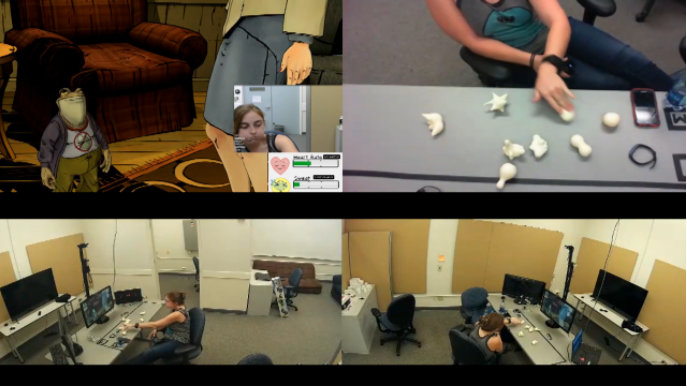
\includegraphics[width=.9\linewidth]{figures/fig1.PNG}
\caption{\label{fig:org35e2737}
Video Recording Setup}
\end{figure}

We also hypothesized that the SEI would provide insights into the more
subtle emotional experiences that were prevalent in this type of
narrative game experience. We further believed that we could use the
use of such an instrument without needing to differentiate between
which instrument was used. For the purposes of this paper, any SEI
usage is an affective event.

Each session was conducted as follows. Players first took a pre-game
questionnaire, with questions covering familiarity with the Fables
comics and whether they've played other titles by Telltale Games. As a
prerequisite to participate in the study, we required that the
participant had never played the game before so their reactions would
be unadulterated; however we learned afterwards that one participant
was familiar with the comic series on which it was based which colored
their knowledge of events and characters. We then calibrated the SEI,
which consists of showing the users a series of 10 photos from the
International Affective Picture System (IAPS) \cite{Lang2005-xi} and
having them indicate with the SEI which association came to their mind
for that particular instrument. We then provided instructions to
participants to play through the entire game while expressing any
thoughts that arose aloud as a think aloud, as well as told them to
use the SEI as much as possible. After noting that the first
participant forgot to use the SEI, we set up a timer to go off as a
reminder periodically. We left the room for the duration of the
gameplay session, only returning in the case of technical
difficulty. Participants were also equipped with the Empatica E4
wristband (ATF) to track their heart rate (HR) and Galvanic Skin
Response (GSR). The facial recognition, Affdex, from ATF was running
as well.  At the end of the session, we conducted a retrospective
think-aloud with the player about how they felt at certain peak
moments of the game, how they felt about various characters, and why
they used specific SEI objects during play. They also took questions
from the IEQ (Immersive Evaluation Questionnaire
\cite{Jennett2008-qs}) and combined them with questions pertaining to
emotion. These provided broad strokes of players retrospective
assessment of their experience.

Once all of the data was collected, we processed the gameplay capture
and cameras to synchronize them using Adobe Premiere Pro to create a
single video for each participant containing gameplay video (with ATF
data as a picture-in-a-picture), top-down view, and left and right
room cameras (see Figure \ref{fig:org35e2737}). We also used the marker feature of
Premiere to hand-annotate features described in the next section due
to the sheer amount of footage, totaling at over 13 hours.
\begin{figure}[htbp]
\centering
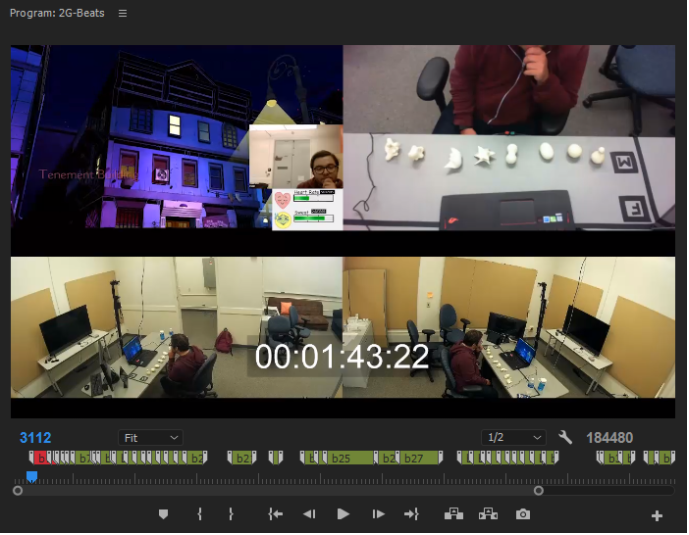
\includegraphics[width=.9\linewidth]{figures/fig2.PNG}
\caption{\label{fig:orgf7d7ebb}
Beat span annotations in Premiere Pro}
\end{figure}

The initial annotations marked locations of features described in the
next section that were identifiable by visual inspection and
unambiguous enough to label without resorting to validation by
inter-annotator agreement methods. We later annotated beats, as the
initial annotation of choice prompts alone proved to vary more than
desired.

At this point we analyzed the choices based on their proximity to
affective signals. This choice-based analysis revealed patterns of
agreement and disagreement as well as emotionally charged and absent
choices. We decided to explore the dataset by charting various
statistical measures of choices. We then did a second pass through the
playthrough videos, side by side, and annotated distinct beats as
described in the next section. While choice points were unambiguous,
they are used in different ways in relation to the story. The next
section presents and discusses the initial features used to annotate
the narrative elements of the playthroughs.


\subsection{Narratological-inspired Annotation Schema}
\label{sec:org43df907}
\emph{TWAU} has three types of gameplay. The first
is the dramatic choice. The second is quicktime events, or
button-pressing sequences that require fast reaction times. The third
is free-roam, most akin to classical adventure games, where the player
can move the player-character about a region of interest and engage
with elements of the environment. We decided to base our analysis of
the narrative content using the notion of a story beat, which has at
its core character interaction and a story value at stake. We also
selected key story events that we believed to have the potential for
player response and which we believed to be directly related to the
primary plot. These provided locations of interest to compare player
traversals and served to align the player data based on a naive
selection of events. Any interruptions are also annotated and excluded
from analysis. The following sections describe each annotation feature
in detail.
\subsection{Beat}
\label{sec:org40218b7}
A beat is defined by Robert McKee as a change in value in the story
which can be brought about by characters, oneself or one's environment
\cite{Mckee1997-ed}. The classic example is one character using a
strategy for something they desire. In \emph{TWAU}, one tense
scene involves a character (Ichabod Crane, deputy mayor) savaging the
player character with blame (beat \#31). This beat ends when the
character turns their attention to another subject and cease
expressing blame. The story value we assigned as an binary-opposition
is Ego/Community, as Crane is attempting to save face at the expense
of serving the community by laying blame on others. During that beat,
the receivers react: in the case of the beat, this reaction is in part
determined by player choice. They can avoid blame, take blame or try
to redirect the conversation. Beats are widely considered an
elementary unit of narrative and were employed in Facade as a means of
organizing and selecting dynamic performance content
\cite{Mateas2002-in}. They can also be classified as either kernel
beats or satellite beats (borrowing from Chatman's terminology
\cite{Chatman1980-rl}). An example of a kernel beat in this sense is
one which must be played for the story to be the same story: for
example, the player must receive a call from Toad providing the
dilemma leading into the fourth chapter. Satellite beats include those
that may not be experienced at all, including alternate endings to
scenarios (whether Bigby roughed up Toad or not, and whether a minor
character dies or not). The fundamental unit of the story beat is
itself central to the the Telltale genre which borrows heavily from
television for its format.

The first three chapters were analyzed for the location of individual
beats. A total of 42 beats were found. There may be that some beats
could be further joined or broken down, but these beats serve the
desired purpose of segmenting content and aligning player data. The
criteria for designating a dramatic exchange as a beat was whether a
single behavior was being pursued by a character directed toward
another character. When either the agent of the action or the behavior
itself changed, a new beat began. There were many segments that were
not beats, including exploration segments. The first fight sequence
(which consisted of Bigby and the Woodsman fighting) was considered a
single beat with the Woodsman as the agent. These include times when
the player-character is roaming around a space and selecting an item
of interest. Sometimes upon selecting an item or option, a beat will
take place with another character also in the room, as is the case in
the business office scene.

Each beat was further tagged with the characters involved, the agent
character and the responding character, as well as the value(s) at
stake. These were frequently truth, justice or compassion as these
were the main themes of the work.
\subsubsection{Dialogue Choices}
\label{sec:org03fbc70}
Choices are the central game mechanic of interest in these games, and
consist of up to four options presented to the player. In timed
prompts, the default option is chosen which is often silence, but can
also be inaction (as is the case when deciding whether to give Faith
money). We apply a simple annotation scheme that records the location
and content of "choice prompts" in the game. We give each choice
prompt a unique ID based on having the same choice strings. In
non-dramatic segments, these may either give the player an option to
choose a major plot branch or simply access expository
information. One particular feature which we could calculated using
the relative timestamps of annotations to one another was the position
of choices relative to their containing beat, if present, as well as
their relative position with respect to the action. In other words,
this heuristic can help to estimate whether a given choice prompt
start the beat as an action, did it continue an action, or was it the
final say in an ongoing beat.

\subsubsection{Story Events}
\label{sec:org2b632ee}
A story event is where an irreversible change occurs which propels the
story forward. This includes information revealed, significant actions
taken and revelations. Some of these events invite player
participation in their outcome, but the presence and content are
mostly fixed. We selected the key events that define the first
episode: rescuing Faith from the Woodsman, finding Faith's Head and
discovering Faith's identity. Each propel Bigby on his quest to solve
the main conflict in the story and each further amplifies the reader's
interest in the form of unanswered questions. Why was Faith being
beaten by the Woodsman? Who was her employer? Who killed her, and why?

\subsubsection{Lenses}
\label{sec:org5cffab0}
One of the major challenges with combining objective and subjective
measures are the models and concepts that are used to connect theory
to practice. In our case, we've developed a set of low-level features
that enable parts of the player experience to be analyzed. In this
section, we describe the interpretive lenses that are used to guide
the application of these featuresets. We use these to analyze the
first three chapters of the game, "Disturbance", "Woodlands" and
"Mirror Mirror". The fourth chapter provides two variants based on
player choice at the end of the third chapter, which presents a
challenge for linearly analyzing beats. The content is largely
identical between playthroughs for the first three chapters. The
following sections go into more detail into how these features will be
used to reveal the relationship between players and the story, as well
as defining the objectives for the various charts and calculus that we
employ.

\textbf{Value}

The first perspective looks at a story as a set of values expressed
through the discourse. In order to interpret a player's perspective of
the values of the story, we need definitions of both value and where
the value can be found in the work itself. According to McKee, scenes
turn on a value change. Each value is expressed as a binary
opposition, where each beat revolves around the expression of one or
the other. The principle values in \emph{TWAU} are \texttt{Community/Ego},
\texttt{Death/Survival}, \texttt{Truth/Lies} and \texttt{Justice/Injustice}. These permeate
the world and are present in every dramatically portrayed scene. By
classifying the annotated beats according to a set of principal value
at stake, the player's affinity for certain values can be estimated.

\textbf{Character}

Certain characters may be more compelling or resonate with players
more than others; Toad's plight as a disadvantaged member of the
community is overshadowed by his acrimonious attitude toward Bigby,
leading to the suspicion that Bigby (and the player) expresses in key
scenes. Another character's grievances are hidden behind a wall of
rage and disrespect. Faith and Snow both are sympathetic and
conflicted. We decided to explore how individual players felt during
scenes in which characters are involved. We did not explore either the
valence or the intensity beyond measuring the frequency of
occurrences. These were used as a measure of engagement with the
content.

\textbf{Choices}

There are two ways we analyzed choices. First, we analyze the
decisions players made for agreement or disagreement. This aids in
determining if there was perception of different outcomes, and also
may indicate segments of gameplay where player preferences differ or
where the experience itself diverged.  We then examine the overall
distribution of choice types in the game according to whether they
were contained in a beat and what position they occupied within it. We
use this timing data as a heuristic to get at what roles choices play
within beats, and which beats are independent of player input.  

These three perspectives represent different layers of narrative
engagement -- at the underlying level of value, where a player takes
on and cares for the values that the story's characters care about, at
the level of character where certain characters may be more or less
engaging than others, and at the level of interactivity. By examining
the content of these narrative elements juxtaposed with differential
measures of player affect, we hope to determine what role the choice
played in the player experience. In the next section we will review
the results of these perspectives.

\section{Results}
\label{sec:org5a44689}
The analysis takes the three lenses and develops charts that describe
that objective for each player. For instance, the character-oriented
analysis would describe a player's affinity for each of the principle
characters in the work in a graphic that links directly to the
annotated dataset. Likewise for values, and likewise for beats. The
primary way in which comparisons are made are two fold. First,
comparisons are made by tallying up lower level features according to
the time windows attributed to each feature. Second, these sums are
normalized in order to highlight inter-player differences on a given
metric. Often characters or values are represented at different levels
throughout the story, and this normalization enables finer details to
be compared. An example of a small scene with a great impact is the
introduction of the antagonist, Grendel, which may fall by the wayside
without this normalization step. The quantitative data consists of a
database that relates each of the inter-player content types to
individual playthrough video timelines. Each row contains the an
integer identifying the type of the annotation (1-12), an ID if
present, and any associated data with the annotation, such as the
content of the choice-prompt or the decision the player made. There
are several secondary tables that collect the independent items,
including the complete set of beats, choices, characters and
values. These are used in a relational-database fashion to perform
queries that correlate elements to one another.

For the purposes of this initial study, we focused only on the first
three chapters for the purposes of the three analyses. The three
chapters provide a classic introduction to a mystery, with the
player-character being called to the scene of a disturbance only to
meet and become attached to the victim. Bigby, The Sheriff of
Fabletown, is confronted with their reputation and past as a violent
character and are stunned by the murder by decapitation of the
character, Faith, just introduced. The third chapter follows the
community and relationships that define Bigby. Overall, we at first
were surprised at the variation in player choices and styles. Players
performed both friendly and aggressive versions of the protagonist and
genuinely engaged with the piece.

\subsubsection{Participants}
\label{sec:org3875209}
Due to technical difficulties we needed to discard one participant's
data (P1) as the physiological measures and camera data were not
complete for the first part of the session. The remaining 6
participants are discussed in the results below. Of the 6 remaining
participants, 5 previously played a Telltale Games title (4 played Walking
Dead, 1 played Sam and Max while 1 played numerous other
titles). There were 3 men (P2, P4, P5) and 3 women (P3, P6 and P7).

\textbf{Emotional Signals}

We define an emotional signal as a time series of measurements by one
of the above means. These are annotated on each player's recorded
video and they represent points in time associated with a peak
expression of one of the measured variables. As discussed before,
these include heart rate, skin conductivity (sweat), facial expression
recognition by ATF (at the peak of an expression detection for a few
seconds), and usage of one of the eight SEI. These signals are at
different times for each player in their respective video due to the
varying nature of parts o the gameplay, and so one of the challenges
is that of aligning one player's emotional signal with the content and
with one another. While we are addressing primarily the content in
this present study, it would be worthwhile to investigate applying
additional measures of insight into the player motivations and
personality in the future. We label each measurement with the type,
the timestamp relative to the player's video and the player's ID.

\textbf{Story Elements}
In the following sections, we will present the analysis according to
the lenses described in the methodology section. These represent the
transformation of objective observations into a narrative-focused
goals for understanding both the player's relationship to the content
and the variation in player experience to one another..

\textbf{Character Affinity}
The goal for a character-oriented analysis is to differentiate players
based on which characters they are most engaged with. Since each
sensory measure is a measure of engagement, the combination, when
associated with characters, can be used to differentiate player
attitudes towards characters. Using the annotations described in
section X, we calculate the player-character affinity chart as
follows: first, sum the total of each measure of affect for all beats
that are tagged with a character for each player, as well as the total
sum of all measures within all beats. Multiply this by the percentage
of time that the relevant beats occupy relative to the total
playtime. Then divide by the average of each character's affinity
measure (in order to enable comparison of characters relative to .

\begin{figure}[htbp]
\centering
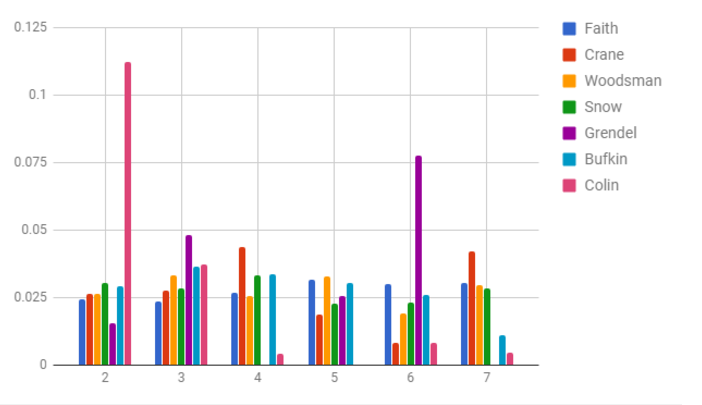
\includegraphics[width=.9\linewidth]{figures/fig3.PNG}
\caption{\label{fig:orge5e1992}
Normalized mapping of players to characters according to affect measures}
\end{figure}


The most prominent element is P2's response to Collin. During the
think aloud, the player reacted strongly to the character and
especially the references from which he was drawn. From this figure,
the two characters that stand out are P6's reaction to Grendel and P7
and P4's response to Crane. Future work will involve charting these
affective responses through player decisions. For instance, in P6's
climax scene, she commits the act of dismembering Grendel's arm. The
unique feeling that a player has toward each character in a narrative
defines their reactions and their enjoyment. Modern television series
produced by Hulu and Netflix often will tailor the series based on fan
responses to characters and relationships. This measure of player to
character relationship may be preliminary, but the concept of creating
a fingerprint of how a player feels about a character indicates that
stories may be able to focus more on measuring and adapting to players
with appropriate modeling.

In the first three chapters, we annotated 50 unique choice sets, using
a simple ID system to distinguish variants of a choice (see Table
X). Each annotation was labeled with a delimited list of elements
including the label itself, the choice the player made, and the choice
options in a predetermined order. Of these, 10 were shown only to some
of the players (the other 40 were shown to all players) in a given
traversal. 47 of these choices were contained within a beat. The first
analysis we conduct is based on proximity of choices to affect
annotations. We consider the count of affect annotations within a time
window starting at the choice itself and lasting either 30 seconds or
until the start of the next choice prompt.

\subsection{Emotional Choices}
\label{sec:orgd19dfdd}
\begin{table*}[htbp]
\caption{\label{tab:org5b03fb1}
Choices with emotion proximity}
\centering
\begin{tabular}{llllll}
\textasciitilde{}ChoiceId\(\approx\) & \texttt{Count} & \texttt{Choice\_X} & \texttt{Choice\_Y} & \texttt{Choice\_A} & \texttt{Choice\_B}\\
\hline
2-2 & 44 & This is your last warning & [threaten him] & \ldots{} & You're drunk\\
3-1 & 35 & Sorry about the car. & How's your insurance? & \ldots{} & Get off the street\\
7-5 & 35 & My job & Don't need advice & \ldots{} & Not my fault\\
2-7 & 33 & HEY! & Will you excuse me a moment & \ldots{} & [Throw him out]\\
19-16 & 31 & Keep it & [Open it] & \ldots{} & It belongs to Lawrence.\\
12-1 & 30 & I'm fine & Fuck off & \ldots{} & I'm not great.\\
\end{tabular}
\end{table*}


In Figure \ref{tab:org5b03fb1}, we show the top 6 choices based on their
proximity to emotional annotations. The number of players that chose
the same response is listed along with the most popular choice.These
reveal some problems with the straightforward approach of mapping
affective annotations onto content: the scene where the top two
options occur are artificially boosted due to the combat sequence that
follows each. While using a time window may help, a type-based
approach to dealing with player affect may be more effective than a
single blanket time window.

\begin{table*}[htbp]
\caption{\label{tab:orgc2d7f73}
Most Agreed Choice Prompts}
\centering
\begin{tabular}{llllll}
\texttt{ChoiceID} & \texttt{D\_ID} & \texttt{Choice\_X} & \texttt{Choice\_Y} & \texttt{Choice\_A} & \texttt{Choice\_B}\\
\hline
13-1 & 2 & Glamour & What do you want? & \ldots{} & The car.\\
7-1 & 2 & Yeah. Get out & C'mon, I'm tired. & \ldots{} & There's only the one.\\
7-7 & 1 & [Give Colin a Drink] & [Take Drink] &  & \\
19-9 & 4 & What toy could have made this mark? & He left the toy for that long? & \ldots{} & The broken lamp was here.\\
19-16 & 2 & Keep it & [Open it] & \ldots{} & It belongs to Lawrence.\\
\end{tabular}
\end{table*}


\ref{tab:orgc2d7f73} tabulates a set of choices that have the most
agreement. All players chose to give the character Colin their drink,
and all characters responded with the most polite response for
\texttt{ChoiceID} \texttt{13-1} and \texttt{7-1}. The \texttt{DecisionID} represents the most popular
choice as an index from the Decision column, which is dynamically
populated.

\subsubsection{Beat Analysis}
\label{sec:org01da7a0}
The next analysis was done based on the breakdown of the first three
chapters into 42 beats. Each beat contained an annotation, which was
summed for each measure and shown in Figure
\ref{fig:org20a5023}. Selection of annotations was for each beat
was extended 15 seconds The overall structure of the first three
chapters is evident, along with selected areas of interest to
different players. The x axis is an ordered sequence of beats from
1-42, whereas the y axis represents the number of affective
annotations in the time window of each beat.

\begin{figure}[htbp]
\centering
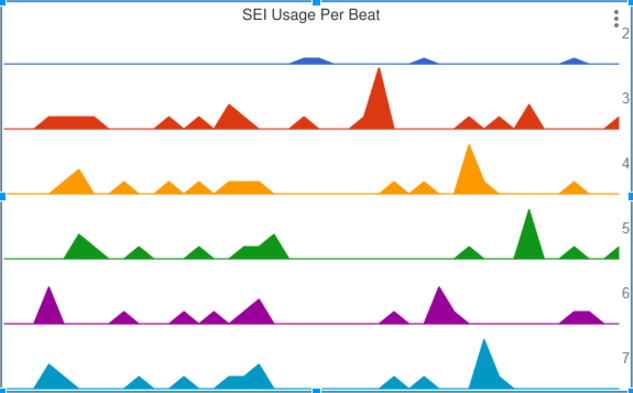
\includegraphics[width=.9\linewidth]{figures/Fig4.PNG}
\caption{\label{fig:org20e409f}
SEI Usage Per Beat}
\end{figure} Charting the SEI reveals differential patterns
amongst several characters more readily than the raw time series data,
or even other measures. It also reveals a spike (A) during the scene
with Colin. More interesting is the variations of focus between player
3 and players 4-7. Reviewing this section of the recording revealed a
spike in valence activations during this time (beat 13, corresponding
to the second fight with the Woodsman). This scene is of interest
because it employs a deceptive strategy that worked exceedingly well
in Player 2s case. During the first fight sequence, the player must
tap a button rapidly to struggle for control of a key weapon. In this
sequence, the same game mechanic is used, but the progress bar that
was present before is artificially diminished no matter what speed the
player presses the button. The first peak in Player 2's signal (B)
indicates that they were thoroughly engaged in the activity and
struggle, more so than the other players, despite not indicating
emotional activity as regularly as the others.  Player 4 and 7 have
spikes in their respective signals for SEI usage at beat \#27, after
Faith's head is revealed, whereas players 3 and 6 react more strongly
during the suspenseful beat prior to the revealing of the murder
victim's severed head. In Figure \ref{fig:org20a5023}, the top SEI
signal (blue) reflects emotional activity after the event at Annotation A,
whereas the physiological measures all peak around the same time at
the moment of the reveal (Annotation B).

\begin{figure}[htbp]
\centering
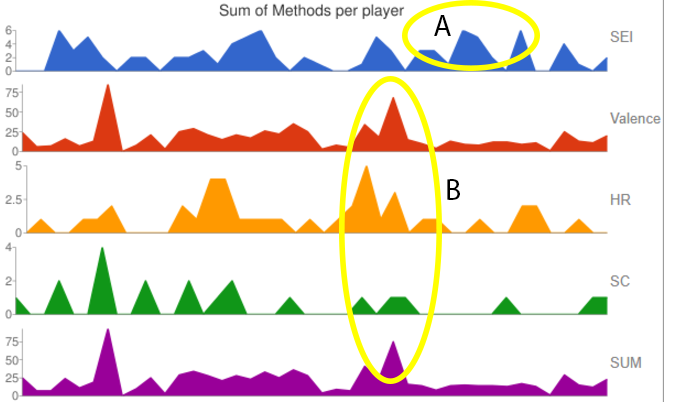
\includegraphics[width=.9\linewidth]{figures/Fig5.PNG}
\caption{\label{fig:org20a5023}
Sum Methods Per Beat}
\end{figure}


We also used the timing information from the beats to analyze the
position of the choice prompts in relation to their containing
beats. Of the 48 choice prompts annotated that occurred within a story
beat, 6 occurred in the first 20\% of a containing beat, and 8 occurred
in the final 20 percent of a containing beat. The remaining 34 took
place somewhere in between. This makes sense as the player-character
or other characters have more of a chance to frame the decision,
whereas an initial choice-prompt would be difficult to keep up.

\subsubsection{Value analysis}
\label{sec:org6109f03}

The final analysis involves examining how players reacted to the main
themes in the story. These are embedded throughout, and so simple
ordered sequences of beats may not reveal a preference toward one
value over another. We came up with the following list of
binary-oppositions to describe the underlying force in each beat:
Justice/Injustice, Ego/Community, Truth/Lies, Nice/Bad, and
Duty/Hedonism. Two beats were not able to be classified, and these
were determined to play a non-dramatic role (one involves a character
asking Bigby about his early guesses as to who the culprit might be,
in order to further solidify Snow's relationship and to pique the
player's interest, and the second is likewise an opportunity for the
player to engage with the speculation regarding the husband of the
victim).

Each beat was labeled with the values, and the sum of each affective
element during each beat was taken. These is demonstrated shown in
\ref{fig:org6c0ff0b}

\begin{figure}[htbp]
\centering
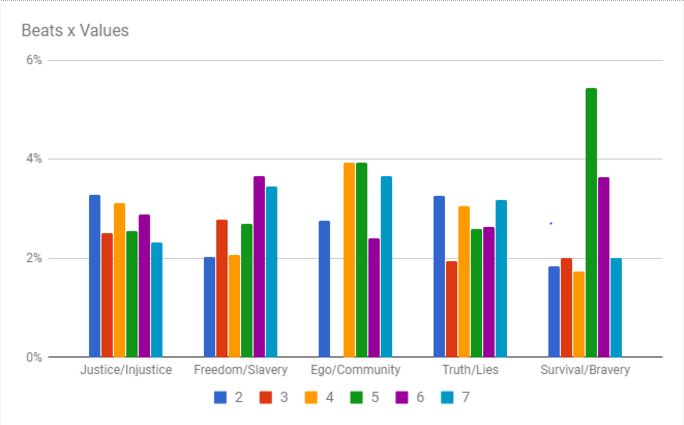
\includegraphics[width=.9\linewidth]{figures/Fig6PNG.PNG}
\caption{\label{fig:org6c0ff0b}
Value-oriented sorting. Each player is sorted according to which value they are most engaged by. Measurement is done by summing the engagements during beats where a value are "at stake"]}
\end{figure}

It is worthwhile to note that P5 stands out from the rest as they
reacted to beats 8, 14 and 19 which concerned survival or
bravery. These beats involve Faith's pursuit of her own self interest
in the face of the Woodsman and the world at large.

\begin{figure}[htbp]
\centering
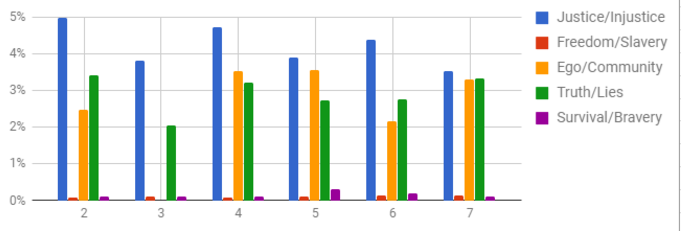
\includegraphics[width=.9\linewidth]{figures/fig7.PNG}
\caption{\label{fig:org68ee32d}
Player-sorted Value Beat Emotional Signals}
\end{figure}

In Figure \ref{fig:org68ee32d}, the distribution of values is not
normalized by subtracting the average value, and so the absolute
relationship between the prominent themes of truth/lies, justice are
contrasted with the less common beats with values of Freedom/Slavery
and Survival/Bravery. These values are further developed later in the
episode and in the series.

The study yielded some patterns that were not immediately apparent
from immersing ourselves in the videos themselves. At times
familiarity with the players and the sheer amount of time-based media
make content-based analysis vital to understanding how players are
experiencing the work.

\section{Discussion}
\label{sec:orgfe21c1b}
While the field of computational modeling of narrative has
not yet advanced to address interactive narratives, this work
represents some of the potential raw materials with which a model can
be evaluated.

Long-form narrative works are difficult to evaluate given the high
demand for skilled interpretation. We are far from a solution for
automated recognition of beats within the context of a modern
adventure game. Our annotation work has demonstrated that smaller
studies can be made more useful when annotated using even naive models
of narrative. 

The current work presented one set of labels and concepts that have
been operationalized to use specific data points. Another set of
binary-opposition pairs may have also suited. Likewise, the exact
specification of what constitutes a beat in drama is fluid and ill
defined in its home discipline of the humanities.

The ways that beats and values functioned did not depend on their
perfect modeling, however. They instead provided a set of handles with
which to examine the data and generated new questions regarding player
interpretations and the value of narrative pacing that we hope to
pursue in future research. To that end, we found that some of the
early decisions about the methods used for recording the experiences
were correct as we developed our techniques. One of the key decisions
made early on was to use analogue video recordings to facilitate
future annotation layers, models and work. This approach is more
exploratory as a result, providing a rich set of data for hypotheses
to be made and tested.

Some of the challenges that arose during the course of this study and
analysis included the knowledge that players brought to bear that may
have interfered with some of the effects. These are not unusual,
however, and we are often in some state of being spoiled as we
encounter stories. Trailers prepare us for what to expect, and the
game itself consistently tells us through music and other means what
will happen next.

\section{Recommendations}
\label{sec:org35e8d4a}
We have some recommendations based on our close analysis of the game
that will assist researchers and practitioners exploring developing
interactive narratives or developing new methods of assessing them.

\begin{enumerate}
\item \emph{Record everything using digital video and high quality
microphones}. As technology improves, the ability to mine
additional details or data out of existing playtests may only be
limited by the quality of the record. We found that once we put in
the work to create a gold-standard playthrough record (by syncing
the various time-based media together, including audio), that
future annotations or development can overlay or replace current
models and techniques.
\item \emph{Vary the theme}. One of the princple observations from the value
and beat based analysis was the sheer variety of functions that
content played in \emph{TWAU}. By keeping each situation the player
encountered fresh and by alternating themes, the game manages to
maintain player interest and keep the theme in the back of their
mind.
\item \emph{Carefully modulate player agency}. We found in analyzing the
location of beats that often having a player-character model a
behavior for the player would set up the player to feel a certain
way about the situation. These actions became adopted by players
despite their not controlling them as they embraced the
player-character as their own.
\end{enumerate}

\section{Conclusion}
\label{sec:org0c7891e}
Combining quantitative measures of affect with content analysis yields
interesting insights into the challenging problem of interactive
narrative analysis. We've demonstrated the application of this method
to a contemporary adventure game as well as demonstrated insights
gleaned from it. Future research should focus on further relationships
between choices and player dispositions, including additional surveys
within the game. Players were not uniform in their expressiveness, or
in their usage of SEI, which may lead to further changes in study
design to encourage players to use the instruments. Also, coding was
laborious and time intensive and would benefit from automation using
either sensors or computer vision approaches.

Despite a small sample size, the study successfully demonstrated a
variety of player choices and responses and demonstrated the benefits
of normalizing structure according to narrative elements. More work
can be done on modeling story elements using a formal model such as
Elson's Story Intention Graph, but it would need to be adapted to
handle the ambiguous and emotional nature of the media. These results
are promising in that the provide evidence that player evaluations of
interactive narratives can benefit from combining content analysis and
existing qualitative methods.

% BALANCE COLUMNS
% \balance{}

% REFERENCES FORMAT
% References must be the same font size as other body text.
\bibliographystyle{SIGCHI-Reference-Format}
\bibliography{references}

\end{document}

%%% Local Variables:
%%% mode: latex
%%% TeX-master: t
%%% End:
